\documentclass[10pt]{report}

\usepackage[utf8]{inputenc}
\usepackage[T1]{fontenc}
\usepackage[francais]{babel}

\usepackage{lmodern}

\usepackage[top=2cm,bottom=1.25cm,right=.75cm,left=2cm]{geometry}

\usepackage{color}
\usepackage{listings}
\lstset{ %
	language=HTML,					% choose the language of the code
	basicstyle=\footnotesize,		% the size of the fonts that are used for the code
	numbers=left,					% where to put the line-numbers
	numberstyle=\footnotesize,		% the size of the fonts that are used for the line-numbers
	stepnumber=1,					% the step between two line-numbers. If it's 1 each line will be numbered
	numbersep=5pt,					% how far the line-numbers are from the code
	backgroundcolor=\color{white},	% choose the background color. You must add \usepackage{color}
	showspaces=false,				% show spaces adding particular underscores
	showstringspaces=false,			% underline spaces within strings
	showtabs=false,					% show tabs within strings adding particular underscores
	frame=single,					% adds a frame around the code
	tabsize=4,						% sets default tabsize to 2 spaces
	captionpos=b,					% sets the caption-position to bottom
	breaklines=true,				% sets automatic line breaking
	breakatwhitespace=false,		% sets if automatic breaks should only happen at whitespace
	title=\lstname,					% show the filename of files included with \lstinputlisting
	escapeinside={\%*}{*)},			% if you want to add a comment within your code
	morekeywords={*,...}			% if you want to add more keywords to the set
}

\usepackage{hyperref}

\title{Projet tuteuré en licence professionnelle\\Compte-rendu de synthèse de la formation}
\author{Julien \bsc{Rosset}}
\date{\today}
\hypersetup {
	pdftitle	=	{Synthèse et bilan final de la formation - Licence Professionnelle DASI en alternance},
	pdfauthor	=	{Julien ROSSET},
	pdfsubject	=	{Compte-rendu de synthèse en licence professionnelle DASI en alternance},
	pdfkeywords	=	{Compte-rendu, synthèse, licence professionnelle},
	pdflang		=	fr_FR,
	pdfborder	=	0 0 0,
	frenchlinks	=	true
}

\usepackage{fancyhdr}
\pagestyle{fancy}

\fancypagestyle{plain}{%
\fancyhf{}
\fancyhead[L]{Julien \bsc{Rosset}}
\fancyhead[C]{Synthèse et bilan finale de formation}
\fancyhead[R]{\today}
\fancyfoot[L]{Université Claude Bernard Lyon 1 - IUT A - Département Informatique - LP DASI A}
\fancyfoot[R]{\thepage}
\setlength{\headsep}{10pt}
\renewcommand{\headrulewidth}{1px}
\renewcommand{\footrulewidth}{1px}}

\fancyhf{}
\fancyhead[L]{Julien \bsc{Rosset}}
\fancyhead[C]{Synthèse et bilan finale de formation}
\fancyhead[R]{\today}
\fancyfoot[L]{Université Claude Bernard Lyon 1 - IUT A - Département Informatique - LP DASI A}
\fancyfoot[R]{\thepage}
\setlength{\headsep}{10pt}
\renewcommand{\headrulewidth}{1px}
\renewcommand{\footrulewidth}{1px}

% Pour la page de garde
\usepackage{color}
\usepackage{changepage}
\usepackage{graphicx}

% Commandes personalisés
\newcommand{\solulog}{\bsc{Solulog}}
\newcommand{\fidit}{\bsc{Fidit}}
\newcommand{\integrale}{\og Intégrale \fg}
\newcommand{\pireus}{\bsc{Pireus}}
\newcommand{\vb}{Visual Basic}

\begin{document}
	%\maketitle
	\begin{titlepage}
	\changepage{+2.5cm}{+5cm}{+0cm}{-2.5cm}{+0cm}{-1cm}{+0cm}{+0cm}{+0cm}

	\begin{center}
		\colorbox{black}{\parbox[top][1.5cm][c]{\textwidth}{
			\begin{center}
				\textcolor{white}{\sffamily{\bfseries{\LARGE{Licence Professionnelle DASI en alternance}}}}
			\end{center}
		}}\\[0.75cm]

		\textsc{Septembre 2010 - Septembre 2011}\\[0.75cm]
		Tuteur enseignant: M. Jean-Michel \bsc{Martiniere}\\[1cm]

		\textsc{\huge \bfseries Synthèse de formation}\\[1cm]

		\emph{Apprenti: }\\Julien \textsc{Rosset}\\[1cm]

		\fbox{\parbox[top][2cm][c]{\textwidth}{\begin{center}\Huge \bfseries Synthèse et bilan final de la formation \end{center}}}\\[1cm]


		\begin{figure}[!htb]
			\begin{center}
				
\includegraphics[scale=.75]{Contenu/Images/Logo_Solulog.png}
			\end{center}
		\end{figure}
		\fbox{\parbox[top][3cm][c]{\textwidth}{\begin{center}\begin{Large}\bsc{Solulog}\end{Large}\\~\\37, rue Montgolfier\\38090 Villefontaine\\
		\vspace{0.5cm}Maître d'apprentissage: M. Philippe \bsc{Perisse}\end{center}}}

		\vfill

		\hrule
		\begin{center}
			Université Claude Bernard - Lyon 1, IUT A
			\begin{figure}[!htb]
				\begin{center}
					
\includegraphics[scale=.25]{Contenu/Images/Logo_IUTA.png}
				\end{center}
			\end{figure}
			Département Informatique\\
			43, Boulevard du 11 novembre 1918 - 69622 Villeurbanne CEDEX\\
			Tél: 04.72.69.21.90
		\end{center}
	\end{center}
\end{titlepage}

	\chapter*{Remerciements}
\addcontentsline{toc}{chapter}{Remerciements}
En premier lieu, je souhaite remercier toute l'équipe des entreprises \solulog{} et \fidit{} pour le merveilleux accueil qu'elles m'ont offert et leurs efforts incessants pour m'intégrer.

Je voudrais également leur exprimer ma gratitude pour m'avoir prêté attention et mis en \oe{uvre} certaines de mes idées afin d'améliorer la qualité du code, et du logiciel d'une manière plus générale.

~

Je souhaite tout autant remercier mes tuteurs, tant à l'IUT qu'en entreprise, pour leur suivi et leurs conseils judicieux.

~

Du côté technique, je tiens à remercier Samuel \bsc{Raposo}, qui a partagé son expérience du module PHP traité dans mon projet tuteuré, ainsi que pour ses nombreuses explications sur l'utilisation des techniques de programmation propres à \solulog.

Je veux également remercier toute l'équipe de développement de \fidit, pour m'avoir si bien accueilli dans leur milieu.


	\renewcommand{\contentsname}{Sommaire}
% 	\setcounter{tocdepth}{3}
	\tableofcontents

	\chapter{Introduction}
La première partie de mon année s'est déroulé au sein de \solulog, sur la période allant du mois de septembre 2010 à la fin du mois d'avril de 2011.

~

Un calendrier donnant la répartition de mes différentes tâches pendant cette période est visible dans l'annexe \ref{calendrier} à la page \pageref{calendrier}.

\paragraph{Plan de la partie}
~

Durant cette période, j'ai été amené à accomplir trois grands projets :
\begin{itemize}
	\item mon projet tuteuré ;
	\item l'intégration des PDF dans \integrale ;
	\item un module commercial pour les entrepôts.
\end{itemize}

~

Afin de tous vous les présenter, je vais détailler chacun de ces projets dans un chapitre. Ensuite, dans un quatrième chapitre, je parlerais de diverse tâches annexes qui m'ont été confiée entre ou même temps que ces projets.


	\section{Présentation}

\subsection{\solulog}

\begin{frame}
	\frametitle{Présentation de \solulog}
	
	\begin{itemize}
		\item TPE : 2 employés + 3 alternants (dont moi)\sautligne
		
		\item Fondé en 2004 par Philippe \bsc{Perisse}
		\item Partenariat avec Fidit en 2006\sautligne
		
		\item \'Edite et distribue \bsc{Intégrale}, suite de logiciels pour :
			\begin{itemize}
				\item Organisation du transport international
				\item Logistique
			\end{itemize}
	\end{itemize}
\end{frame}

\subsection{Environnement}

\begin{frame}
	\frametitle{Présentation de l'environnement}
	
	\begin{itemize}
		\item Accès TSE à une session distante pour le travail\sautligne
		
		\item Microsoft SQL Server 2005 pour les données
		\item Microsoft \bsc{Access} 2003 pour les interfaces
		\item Visual Basic 6 pour les traitements\sautligne
		
		\item Pour le projet :
			\begin{itemize}
				\item Langage PHP
				\item Web services avec SOAP
			\end{itemize}
	\end{itemize}
\end{frame}

\chapter{Le projet tuteuré}
Bien qu'il ai déjà fait l'objet d'un compte rendu détaillé de réalisation, je ne peux pas faire une synthèse de mon année sans le mentionner.

~

Bien évidemment, ce chapitre à pour but de donner seulement un aperçu de mon projet tuteuré. Si vous souhaiter un savoir plus à son propos, je vous conseille de vous référer au-dit compte rendu détaillé, disponible ici : \url{https://github.com/downloads/darkelfe/Rapports/LicenceProfesionnelleDASI_ProjetTuteure_Rapport.pdf}.

~

Le projet tuteuré m'a occupé pendant presque un mois complet : octobre 2010.

\section{Présentation}
\subsection{Origine du module}
Parmi les nombreuses fonctionnalités proposées par \integrale, il existe plusieurs possibilités d'envoi automatique de documents. En effet, l'organisation du transport international nécessite l'envoi de divers documents officiels, par exemple à la douane, ou à la compagnie maritime pour réserver des emplacement sur un bateau, etc. A l'ère de l'informatique, tous ces documents sont désormais électroniques mais un problème majeur reste : il peuvent être très compliqués à écrire.

C'est pour cette raison qu'\integrale{} propose d'écrire automatiquement ces documents, en y incluant toutes les informations nécessaires, et de les envoyer à son destinataire par un simple clic sur un bouton.

~

Dans le cadre du projet tuteuré, nous devons nous concentrer sur un seul de ces documents : le \emph{Boat Landing}, généralement abrégé en
\og BL \fg. Il s'agit d'un fichier émit à l'attention de la compagnie maritime qui détaille le contenu d'un projet : nombre et propriétés des conteneurs\footnote{Ici, il est fait référence aux conteneurs \emph{maritimes}, c'est-à-dire de grandes boites rectangulaires métalliques.}, poids et volume des marchandises qui sont dedans, etc.

Une des particularité de ce fichier, c'est ça totale illisibilité par un être humain. Les informations qu'il contient doivent respecter une norme particulière qui ne facilite pas la lecture.

~

Pour simplifier le travail de nos clients, \solulog{} à donc décider de créer un module qui crée ce fichier puis l'envoi par internet.

\subsection{\pireus}
Tout commence donc en 2006 avec Alexandre, qui est chargé de ce travail. Vu que \solulog{} souhaite pouvoir vendre ce futur module indépendamment de \integrale, il est décidé que le module, nommé \emph{\pireus}, sera écrit en PHP, avec seulement un petite partie en \vb{} pour transmettre les données nécessaire à la création du fichier.

~

Quelques temps plus tard, le module est prêt et mis en service. Les années passent et en 2009, Alexandre, le responsable du module, quitte \solulog. \pireus fonctionnant parfaitement, les choses reste comme cela.

Mais à la fin de la même année, \solulog{} se trouve dans l'obligation de modifier ce module pour y intégrer de nouvelles fonctionnalités. Or, il y a un problème assez gênant : personne, au sein de \solulog, ne maitrise le PHP. Finalement, c'est Samuel qui se charge des modifications. Malgré l'aide d'Alexandre, Samuel ne peut appréhender la totalité du module et effectue seulement les modifications demandées.

\vfill

\subsection{Objectifs}
C'est cet événement qui va pousser \solulog{} à réfléchir au problème. Il va finalement en ressortir que le module doit être entièrement réécrit en \vb{} et intégré à \integrale.

~

Mon arrivée en 2010 leur donne l'occasion d'effectuer cette tâche. Je suis donc chargé, à titre de projet tuteuré, de réécrire entièrement un module PHP en \vb. Je dois également en profiter pour écrire une documentation complète sur mon module, afin de simplifier les modifications ultérieures.

\section{Déroulement du projet}
\subsection{Étude de l'existant}
Les premiers temps de mon projet tuteuré ont consisté à étudier le code du module existant, afin de comprendre comment celui-ci fonctionnait. Malheureusement, plusieurs problèmes sont venu compliquer l'affaire.

~

Premièrement, le code n'est pas documenté et peu commenté. Or, l'objectif principale de cette étude, c'est identifier la structure du fichier final et repérer quelle sont les informations stockée dedans. Sans une documentation qui indique quels segments\footnote{ici, le terme de \emph{segment} désigne un fragment du fichier final : les BL sont intégralement constitués des \emph{segments}.} comportent quelles informations, il devient difficile de comprendre le processus qui permet de passer des données de départ au résultat final. La seule documentation que j'avais à ma disposition est celle fournie par la norme des fichiers de BL : un énorme document pas facilement compréhensible, qui contient de nombreuse informations qui ne sont pas utilisées par \pireus.

Le second problème, c'est que \pireus{} est écrit de manière générique, c'est à dire qu'il est prévu pour être facilement adapté à des fichiers autres que les BL. Même si c'est un point que \solulog{} ne souhaitait pas conserver, j'ai du faire le tri entre le code \og utile \fg, qui agit réellement sur les données et celui chargé de mettre en place le côté générique du code.

Et enfin, le troisième problème se situe au niveau de l'échange des données entre \integrale, écrit en \vb, et le module en PHP. \pireus{} est écrit comme un programme indépendant, c'est à dire qu'il peut recevoir les informations qui lui sont nécessaire de n'importe quelle source. Pour que cela soit possible, il a fallu construire un support pour les données qui puisse être utilisé par tous. C'est dans ce bus que le \pireus{} utilise un ensemble de fonctions appelée \og SOAP \fg. Malheureusement, lorsque j'ai commencé mon projet tuteuré je ne connaissais absolument SOAP, j'ai donc dû m'adapter ce code pour le moins étrange.

~

Le cumul de ces problèmes m'a totalement bloqué car ils rendaient la compréhension du code totalement impossible. Après avoir réfléchi, j'ai décider de changer de méthode pour approcher le module et est décidé d'utiliser la \emph{rétro-ingénierie}.

~

\fbox{\begin{minipage}[c]{18.1cm}
	\begin{bf}La rétro-ingénierie\end{bf}

	La rétro-ingénierie est un technique, souvent utilisée en informatique mais aussi dans d'autres domaines, qui consiste à partir du résultat d'un processus pour retrouver le point de départ.
\end{minipage}}

~

J'ai donc pris un fichier de BL et en faisant le parallèle avec les informations de départ, j'ai enfin pu identifier une majorité des segments et de leur construction. En ce concerne la partie pas encore identifiée, cela c'est fait au fur et à mesure que je réécrivais le module : je comparais mon travail au module \pireus.

\subsection{Création du message}
L'étape suivante, c'est de réécrire le module. Le processus à un ordre d'exécution très précis. Afin de simplifier l'ensemble, je l'ai découpé en plusieurs tâches.

\subsubsection{Lecture des données}
La première chose à faire, c'est de récupérer l'ensemble des données nécessaires à l'écriture d'un BL. Ces valeurs devant être stockée en mémoire le temps du processus, j'ai créé plusieurs structures de données. Ma première tentative n'ayant pas satisfait mon supérieur, j'ai du créer de nouvelles structures plus conformes au souhaits de mon tuteur entreprise.

Une fois les données prêtes à être stockées, la lecture elle-même à commencée. Rien de très compliqué : les données sont extraites de la base de donnée, quelques vérifications de routine puis on stocke le résultat dans la variable qui lui correspond.

\vfill

\subsubsection{Tests sur les données}
Comme je l'ai déjà mentionné, les BL sont régis par des règles et des restriction très précise. Par exemple, le nom du destinataire ne peut pas dépasser trente-cinq caractères, etc. Donc, avant d'écrire le message de BL, il faut mener plusieurs tests pour vérifier que toutes les données sont correctes et prêtes à être insérer dans un BL.

La seule difficulté à été de fusionner les tests effectué par \integrale{} après la lecture, et ceux fait par \pireus{} avant l'écriture du message.


	\part{Synthèse : de septembre 2010 à avril 2011}

\chapter{Introduction}
La première partie de mon année s'est déroulé au sein de \solulog, sur la période allant du mois de septembre 2010 à la fin du mois d'avril de 2011.

~

Un calendrier donnant la répartition de mes différentes tâches pendant cette période est visible dans l'annexe \ref{calendrier} à la page \pageref{calendrier}.

\paragraph{Plan de la partie}
~

Durant cette période, j'ai été amené à accomplir trois grands projets :
\begin{itemize}
	\item mon projet tuteuré ;
	\item l'intégration des PDF dans \integrale ;
	\item un module commercial pour les entrepôts.
\end{itemize}

~

Afin de tous vous les présenter, je vais détailler chacun de ces projets dans un chapitre. Ensuite, dans un quatrième chapitre, je parlerais de diverse tâches annexes qui m'ont été confiée entre ou même temps que ces projets.

% \chapter{Le projet tuteuré}
Bien qu'il ai déjà fait l'objet d'un compte rendu détaillé de réalisation, je ne peux pas faire une synthèse de mon année sans le mentionner.

~

Bien évidemment, ce chapitre à pour but de donner seulement un aperçu de mon projet tuteuré. Si vous souhaiter un savoir plus à son propos, je vous conseille de vous référer au-dit compte rendu détaillé, disponible ici : \url{https://github.com/downloads/darkelfe/Rapports/LicenceProfesionnelleDASI_ProjetTuteure_Rapport.pdf}.

~

Le projet tuteuré m'a occupé pendant presque un mois complet : octobre 2010.

\section{Présentation}
\subsection{Origine du module}
Parmi les nombreuses fonctionnalités proposées par \integrale, il existe plusieurs possibilités d'envoi automatique de documents. En effet, l'organisation du transport international nécessite l'envoi de divers documents officiels, par exemple à la douane, ou à la compagnie maritime pour réserver des emplacement sur un bateau, etc. A l'ère de l'informatique, tous ces documents sont désormais électroniques mais un problème majeur reste : il peuvent être très compliqués à écrire.

C'est pour cette raison qu'\integrale{} propose d'écrire automatiquement ces documents, en y incluant toutes les informations nécessaires, et de les envoyer à son destinataire par un simple clic sur un bouton.

~

Dans le cadre du projet tuteuré, nous devons nous concentrer sur un seul de ces documents : le \emph{Boat Landing}, généralement abrégé en
\og BL \fg. Il s'agit d'un fichier émit à l'attention de la compagnie maritime qui détaille le contenu d'un projet : nombre et propriétés des conteneurs\footnote{Ici, il est fait référence aux conteneurs \emph{maritimes}, c'est-à-dire de grandes boites rectangulaires métalliques.}, poids et volume des marchandises qui sont dedans, etc.

Une des particularité de ce fichier, c'est ça totale illisibilité par un être humain. Les informations qu'il contient doivent respecter une norme particulière qui ne facilite pas la lecture.

~

Pour simplifier le travail de nos clients, \solulog{} à donc décider de créer un module qui crée ce fichier puis l'envoi par internet.

\subsection{\pireus}
Tout commence donc en 2006 avec Alexandre, qui est chargé de ce travail. Vu que \solulog{} souhaite pouvoir vendre ce futur module indépendamment de \integrale, il est décidé que le module, nommé \emph{\pireus}, sera écrit en PHP, avec seulement un petite partie en \vb{} pour transmettre les données nécessaire à la création du fichier.

~

Quelques temps plus tard, le module est prêt et mis en service. Les années passent et en 2009, Alexandre, le responsable du module, quitte \solulog. \pireus fonctionnant parfaitement, les choses reste comme cela.

Mais à la fin de la même année, \solulog{} se trouve dans l'obligation de modifier ce module pour y intégrer de nouvelles fonctionnalités. Or, il y a un problème assez gênant : personne, au sein de \solulog, ne maitrise le PHP. Finalement, c'est Samuel qui se charge des modifications. Malgré l'aide d'Alexandre, Samuel ne peut appréhender la totalité du module et effectue seulement les modifications demandées.

\vfill

\subsection{Objectifs}
C'est cet événement qui va pousser \solulog{} à réfléchir au problème. Il va finalement en ressortir que le module doit être entièrement réécrit en \vb{} et intégré à \integrale.

~

Mon arrivée en 2010 leur donne l'occasion d'effectuer cette tâche. Je suis donc chargé, à titre de projet tuteuré, de réécrire entièrement un module PHP en \vb. Je dois également en profiter pour écrire une documentation complète sur mon module, afin de simplifier les modifications ultérieures.

\section{Déroulement du projet}
\subsection{Étude de l'existant}
Les premiers temps de mon projet tuteuré ont consisté à étudier le code du module existant, afin de comprendre comment celui-ci fonctionnait. Malheureusement, plusieurs problèmes sont venu compliquer l'affaire.

~

Premièrement, le code n'est pas documenté et peu commenté. Or, l'objectif principale de cette étude, c'est identifier la structure du fichier final et repérer quelle sont les informations stockée dedans. Sans une documentation qui indique quels segments\footnote{ici, le terme de \emph{segment} désigne un fragment du fichier final : les BL sont intégralement constitués des \emph{segments}.} comportent quelles informations, il devient difficile de comprendre le processus qui permet de passer des données de départ au résultat final. La seule documentation que j'avais à ma disposition est celle fournie par la norme des fichiers de BL : un énorme document pas facilement compréhensible, qui contient de nombreuse informations qui ne sont pas utilisées par \pireus.

Le second problème, c'est que \pireus{} est écrit de manière générique, c'est à dire qu'il est prévu pour être facilement adapté à des fichiers autres que les BL. Même si c'est un point que \solulog{} ne souhaitait pas conserver, j'ai du faire le tri entre le code \og utile \fg, qui agit réellement sur les données et celui chargé de mettre en place le côté générique du code.

Et enfin, le troisième problème se situe au niveau de l'échange des données entre \integrale, écrit en \vb, et le module en PHP. \pireus{} est écrit comme un programme indépendant, c'est à dire qu'il peut recevoir les informations qui lui sont nécessaire de n'importe quelle source. Pour que cela soit possible, il a fallu construire un support pour les données qui puisse être utilisé par tous. C'est dans ce bus que le \pireus{} utilise un ensemble de fonctions appelée \og SOAP \fg. Malheureusement, lorsque j'ai commencé mon projet tuteuré je ne connaissais absolument SOAP, j'ai donc dû m'adapter ce code pour le moins étrange.

~

Le cumul de ces problèmes m'a totalement bloqué car ils rendaient la compréhension du code totalement impossible. Après avoir réfléchi, j'ai décider de changer de méthode pour approcher le module et est décidé d'utiliser la \emph{rétro-ingénierie}.

~

\fbox{\begin{minipage}[c]{18.1cm}
	\begin{bf}La rétro-ingénierie\end{bf}

	La rétro-ingénierie est un technique, souvent utilisée en informatique mais aussi dans d'autres domaines, qui consiste à partir du résultat d'un processus pour retrouver le point de départ.
\end{minipage}}

~

J'ai donc pris un fichier de BL et en faisant le parallèle avec les informations de départ, j'ai enfin pu identifier une majorité des segments et de leur construction. En ce concerne la partie pas encore identifiée, cela c'est fait au fur et à mesure que je réécrivais le module : je comparais mon travail au module \pireus.

\subsection{Création du message}
L'étape suivante, c'est de réécrire le module. Le processus à un ordre d'exécution très précis. Afin de simplifier l'ensemble, je l'ai découpé en plusieurs tâches.

\subsubsection{Lecture des données}
La première chose à faire, c'est de récupérer l'ensemble des données nécessaires à l'écriture d'un BL. Ces valeurs devant être stockée en mémoire le temps du processus, j'ai créé plusieurs structures de données. Ma première tentative n'ayant pas satisfait mon supérieur, j'ai du créer de nouvelles structures plus conformes au souhaits de mon tuteur entreprise.

Une fois les données prêtes à être stockées, la lecture elle-même à commencée. Rien de très compliqué : les données sont extraites de la base de donnée, quelques vérifications de routine puis on stocke le résultat dans la variable qui lui correspond.

\vfill

\subsubsection{Tests sur les données}
Comme je l'ai déjà mentionné, les BL sont régis par des règles et des restriction très précise. Par exemple, le nom du destinataire ne peut pas dépasser trente-cinq caractères, etc. Donc, avant d'écrire le message de BL, il faut mener plusieurs tests pour vérifier que toutes les données sont correctes et prêtes à être insérer dans un BL.

La seule difficulté à été de fusionner les tests effectué par \integrale{} après la lecture, et ceux fait par \pireus{} avant l'écriture du message.

% \chapter{Gestion des factures aux format PDF}
\section{Présentation}
bla bla bla

\section{Impression au format PDF}
\subsection{Présentation}
bla bla bla

\section{Génération automatique de facture}
\subsection{Présentation}
bla bla bla

% \chapter{Gestion commerciale d'un entrepôt}
\section{Présentation}
bla bla bla

\section{Étude avec UML}
bla bla bla

\section{Réalisation du module}
bla bla bla

\section{Ce qu'il reste à faire}
bla bla bla

% \chapter{Tâches annexes}
Avant d'aborder la seconde partie de mon année, je vais parler brièvement des courts projets que j'ai également mené en même temps que les projets détaillés précédemment.

\section{Ajustement automatique de la taille}
\subsection{Présentation}
Un des désavantages de réaliser nos interfaces avec \bsc{Access} 2003, c'est que celui-ci ne sait pas s'adapter automatiquement à la taille de la fenêtre. C'est-à-dire que quelle que soit la taille de votre écran, l'ensemble a toujours la même taille.

De nos jours, les écrans sont de plus en plus grand. Mais il existe encore des écrans plus petits. Pour que \integrale{} puisse s'adapter à tous les écrans, ses formulaires ont été réalisées pour de petits écrans. Le problème survient lorsqu'on lance le programme avec un grand écran : la fenêtre affichée n'occupe qu'un fragment de l'écran. De plus, les objets présents dedans sont assez petits, ce qui les rends difficile d'accès.

~

Afin de résoudre ce problème, \solulog{} m'a chargé de créer un système capable de redimensionner automatiquement le contenu d'un formulaire.

\subsection{Réalisation}
Avant même de réaliser l'agrandissement des formulaires, j'ai cherché un moyen d'obtenir le facteur d'agrandissement dont j'avais besoin.

~

La première chose à laquelle j'ai pensé, c'est récupérer les dimensions de l'écran actuel et de calculer le facteur par rapport à la taille initiale des fenêtres. Le problème, c'est que le \vb{} est trop ancien pour disposer de fonctions permettant de connaître les caractéristiques de l'écran connecté. J'ai continué à chercher et me suis finalement rendu à l'évidence : il n'existait qu'un seul moyen pour m'en sortir. Heureusement, il s'agit d'une solution très simple : l'utilisateur renseigne le facteur \og à la main \fg.

Par chance, la plupart des d'utilisateurs travaillent sur un poste fixe, toujours avec le même écran. Avec l'aide de mon supérieur, j'ai ajouté un réglage permettant à chaque utilisateur de régler ce facteur.

~

Ensuite, il fallait passer au redimensionnement du formulaire lui-même. De ce côté-là, le \vb{} est bien fait : il dispose de nombreuses fonctions permettant de parcourir l'ensemble des éléments d'un formulaire.

Le principe est simple : parcourir chaque éléments du formulaire, et pour chacun, multiplier ses dimensions par le facteur. Il faut également appliquer le facteur à la position de l'objet : évite que tous les éléments se retrouvent tous les uns sur les autres. Ensuite, si l'élément en question dispose d'un texte (de base ou saisi par un utilisateur), je multiplie la taille de sa police de caractère.

~

Globalement, tout s'est bien passé à l'exception des onglets. Ceux-ci ont un fonctionnement un peu différent et j'ai mis un long moment à identifier et corriger le problème.

\section{Système de traduction des fenêtres}
\subsection{Présentation}
Pour le moment, \integrale{} est un produit entièrement français, il est donc écrit en français. Mais \solulog{} souhaiterai le vendre à l'étranger, ou le mettre en place dans des filières étrangères de nos clients. Le problème qui apparaît immédiatement est celui de la langue. Comme pour la majorité des programmes, il est impossible d'écrire une version du programme par langue. Il fallait donc un système multi-langue, dont la mise en place m'a été confié.

~

Mon supérieur avait déjà une ébauche d'idée sur le sujet : les traductions des textes seraient stockées dans un simple fichier au format INI\footnote{Il s'agit d'un format de fichier simple et connu, qui associe une valeur à une clé.}.

\subsection{Réalisation}
Le chemin pour faire cela était donc tout tracé. Me basant sur mon programme d'ajustement automatique des tailles, je parcours finalement l'ensemble des éléments du formulaire et s'il dispose d'un texte, je recherche celui-ci dans le fichier INI associé à la langue. Si je lui trouve une valeur associée, je la récupère pour la mettre à la place du texte existant.

~

La seule difficulté, en théorie, était de lire les fichiers INI. Mais le \vb{} dispose de nombreuses fonctions permettant d'accéder à un fichier de ce genre. Grâce à un autre exemple présent dans \integrale, j'ai facilement pu comprendre comment lire un fichier INI et mettre moi-même en pratique ces fonctions.

\section{Écriture linéaire d'un nombre}
\subsection{Présentation}
Ce mini-projet c'est déroulé pendant que je travaillais sur le module de gestion commerciale détaillé au chapitre \ref{gestion_commerciale}.

~

Mon maître d'apprentissage en entreprise était à la recherche d'une fonction qui lui permette d'obtenir l'écriture linéaire d'un nombre. Par exemple, transformer \og 142 \fg{} en \og cent quarante-deux \fg.

Je me suis donc lancé dans l'étude d'une fonction de ce genre. Il s'est avéré qu'il n'existe pas, en \vb, de fonction permettant cela. J'ai donc décidé  de l'écrire moi-même.

\subsection{Réalisation}
Dans un premier temps, j'ai cherché un site récapitulant l'ensemble des règles de français conditionnant l'écriture linéaire d'un nombre (qui prend des \og s \fg{} et quand, etc.). Grâce à cela, j'ai écrit une première fonction qui découpe le nombre obtenu par groupes de trois chiffres. Ensuite, je convertis chacun de ces groupes en son expression linéaire. Pour terminer le travail, il ne reste plus qu'à regrouper les expressions avec les séparateurs correspondant (milliers, millions, etc.).




% Calendrier => annexes
%
% plan prévu :
% - projet tuteuré
% - factures pdf
% 	- impression
% 	- programme génération automatique
% - gestion commerciale
%
% - tâches annexes
% 	- redimensionnement automatique
% 	- traduction
% 	- conversion littérale (int => nombre écrit)

	\part{Synthèse : de mai 2011 à septembre 2011}

\chapter{Introduction}
La première partie de mon année s'est déroulé au sein de \solulog, sur la période allant du mois de septembre 2010 à la fin du mois d'avril de 2011.

~

Un calendrier donnant la répartition de mes différentes tâches pendant cette période est visible dans l'annexe \ref{calendrier} à la page \pageref{calendrier}.

\paragraph{Plan de la partie}
~

Durant cette période, j'ai été amené à accomplir trois grands projets :
\begin{itemize}
	\item mon projet tuteuré ;
	\item l'intégration des PDF dans \integrale ;
	\item un module commercial pour les entrepôts.
\end{itemize}

~

Afin de tous vous les présenter, je vais détailler chacun de ces projets dans un chapitre. Ensuite, dans un quatrième chapitre, je parlerais de diverse tâches annexes qui m'ont été confiée entre ou même temps que ces projets.

\chapter{Tampon-FLASH}
bla bla bla
\subsection{Vente en Plus}

\begin{frame}
	\frametitle{Réécriture du module}

	\begin{description}
		\item[Description :] Administration pure
			\begin{itemize}
				\item Gestion contenu\sautligne

				\item Module recherche
				\item Import / Export documents
			\end{itemize}~

		\item[État : ] Pas démarré
			\begin{itemize}
				\item Délais courts
				\item Projet \og standard \fg
			\end{itemize}
	\end{description}
\end{frame}


	\part{Bilans}

\chapter{Bilan personnel}
Cette année, en termes de compétences, m'a apporté bien plus que je n'aurais pu l'imaginer.

\section{Solulog}
Parlons du \vb. Il s'agit d'un premier langage que j'ai appris. Malgré ma grande pratique de celui-ci par la passé, les années ont fini par effacer un partie de lui de ma mémoire. C'est avec un immense plaisir que j'ai repris l'étude et la mise en œuvre de ce langage cette année.

~

Grâce au \vb{} et surtout à \integrale, j'ai eu l'occasion de côtoyer d'autres technologie informatique. Le meilleur exemple qui me vient, c'est le PHP, tant par le biais de \pireus{} que dans la réalisation de sites web avec \fidit.

J'ai également découvert les \emph{Boat Landing} et la norme IFTMIN D99B. Malgré la complexité de celle-ci, j'ai énormément apprécié d'avoir pu mettre en place un tel système et de le voir mis en service chez plusieurs clients.

~

En ce qui concerne l'impression en PDF, l'utilisation d'une imprimante virtuelle comme programme tiers à été extrêmement révélateur pour moi. Cet aspect du projet ma donné l'occasion d'écrire un module complet sur un domaine dans lequel je suis le seul expert de \solulog. Il est satisfaisant et également responsabilisant de savoir que tout le reste de l'entreprise repose entièrement et uniquement sur vous pour cette technologie en particulier.

~

Le module de gestion commerciale c'est également montré utile, notamment dans le cas des entrepôts. Le module, tel qu'il est construit m'a obligé à penser sur deux niveaux en même temps. D'un premier côté, il doit être vu comme un programme à part entière. Il dispose de ses propres réglages et chaque donnée se recoupe. J'ai vraiment eu l'impression d'écrire un programme totalement nouveau.

Le second côté porte sur les liens que doit avoir ce programme avec le module de gestion d'entrepôts. Ce dernier ne doit pas être modifié de n'importe quelle manière. Les liens vers la gestion commerciale doivent venir s'y intégrer sans perturber son fonctionnement si le module en question est absent. Il s'agit d'améliorer un code existant sans le modifier de manière trop radicale.

~

Ces deux projets, par leurs connexions avec les factures m'ont poussé à m'intéresser à la manière dont \integrale{} imprime ses factures. Cela m'a fait découvrir les \og états \fg{} d'\bsc{Access} et m'a plongé un peu plus au cœur de ce logiciel.

\section{Fidit}
Bien que cet aspect de mon année soit arrivé un peu à l'improviste, cela m'a donné l'occasion de découvrir la gestion de projet sous un angle inédit. Après avoir vu Jean-Michel \bsc{Colas} la pratiquer chaque jour se révèle une expérience très différente de l'étude théorique vue en cours.

~

Cela m'a également fait plonger à l'intérieur des techniques de développement de \fidit. J'y ai découvert de nombreuses technologies (système de paiement en ligne, le langage javascript) ainsi que des méthodes de programmation innovantes.

\chapter{Bilan professionnel}
Du coté de l'entreprise, je pense avoir parfaitement réussi à mener mes objectifs à bien. En effet, il existe maintenant un module parallèle à \pireus, mais entièrement en \vb. En outre, il dispose désormais de davantage de fonctionnalités que le module originel (NVOCC, etc.)

Ce nouveau module est désormais en place chez plusieurs clients et semble fonctionner pour le mieux. Les objectifs semblent donc être remplis.

~

Ma curiosité naturelle m'a poussé, tout au long de ce projet, à étudier des aspects du \vb{} plus poussés que nécessaire. Certains d'entre eux m'ont semblé être utiles pour \integrale, et je les ai donc proposés à \solulog, qui les a parfois mis en \oe{uvre}.

~

J'ai également pu apporter une certaine expertise en programmation et pour améliorer le code existant. J'ai su identifier des fragments de code récurrents et les factoriser dans des fonctions.

~


Du point de vue de mon orientation professionnelle, ce projet m'a grandement conforté dans l'idée que le développement informatique est une voie qui me plaît. Je ne regrette aucun moment passé à réfléchir au code d'Alexandre ou à résoudre un problème technique.

J'ai pu également me prouver que je ne m'ennuie pas malgré plusieurs semaines consécutives sur un même projet. Chaque étape de la création d'un programme possède une diversité qui lui est propre, provoquant un renouvellement constant de l'intérêt.

De plus, j'ai appris que même en travaillant avec un langage qui \og vieillit \fg, je peux prendre beaucoup de plaisir.
\chapter{Perspectives d'avenir}
Le mois de septembre 2011 arrive et il est temps de faire le point sur mon année. Globalement, je crois que \solulog{} tout autant que \fidit{} ont apprécié ma participation, car les deux entreprises souhaitent me conserver pour les années à venir.

~

Bien qu'aucun jugement officiel sur cette affaire n'est été émis (ça sera le cas le 16 septembre), il semblerais que \fidit{} veuille définitivement m'intégrer à son équipe.

Mon expérience conjointe au sein des deux entreprises est un atout majeur pour moi. Je serait engagé et employé à temps plein par \fidit, mais également envoyé de manière régulière au sein de \solulog{} pour les aider au développement de \integrale.

~

En ce qui me concerne, je serais absolument enchanté de pouvoir poursuivre cette incroyable expérience avec eux, ce travail me donnant aussi la possibilité de changer régulièrement d'environnement et aussi de langage.



	\chapter*{Conclusion}
\addcontentsline{toc}{chapter}{Conclusion}
bla bla bla

	\appendix
	\part{Annexes}
\chapter{Fichier exemple de BL}

Voici un exemple de fichier BL :
\label{ex_bl}
\begin{lstlisting}
UNB+UNOC:3+AMM:ZZZ+INTTRA:ZZZ+110106:1051+I110106105140'
UNH+M110106105140+IFTMIN:D:99B:UN'
BGM+340+M101028101317::000006+5'
DTM+137:201101061051:203'
TSR+30+2'
FTX+AAI+++VRAIMENT PAS'
FTX+AAI+++IMPRIMME ??'
FTX+BLC+++CONSULTER SITE RENAULT EN '
FTX+BLC+++LIGNE'
FTX+BLC+++EXPLOSIFS VISIBLE SUR '
FTX+BLC+++WIKIPEDIA'
FTX+BLC+++WHOAAAAAAAAAAAAAAAAAAAAA'
FTX+BLC+++END'
FTX+BLC+++THIS IS THE END'
FTX+CCI++MFS+5:US'
CNT+7:6207:KGM'
CNT+11:707'
CNT+15:190:MTQ'
CNT+16:2'
LOC+57+USEKQ::6:MONTICELLO, KY [WAYNE COUNTY AIRPORT]+US'
LOC+73+FRMRS::6:MARSEILLE+FR'
DTM+95:201101061051:203'
RFF+BN:BOOKING'
RFF+FF:070218'
CPI+4++C'
TDT+20+NO_VOYAGE+1++MAER:172+++:::GERDM'
LOC+88+NLRTM::6:ROTTERDAM+NL'
LOC+9+NLRTM::6:ROTTERDAM+NL'
LOC+11+USEKQ::6:MONTICELLO, KY [WAYNE COUNTY AIRPORT]+US'
LOC+7+FRMRS::6:MARSEILLE+FR'
NAD+CA+MAER:160:86++MAERSK+LE PORT:13000 MARSEILLE:FRANCE'
NAD+CN+++RENAULT TIN YANG:SUR LE PORT+7 ALLEE DU BOIS VERT:CENTRE-VILLE:TAIWAN+++456+US'
NAD+CZ+++RENAULT DESCHAMPS:ZONE PORTUAIRE+14 RUE LOUIS ARMAND:ZI LA MOUCHE:95130 LE PLESSIS BOUCHARD:FRANCE'
NAD+FW+AMMFRMB:160:86++RAPID TRANSPORT+BAT 3A - PARC CLUB DES AYGALADES:35 BD CAPITAINE GEZE:13014 MARSEILLE:FRANCE'
NAD+NI+++DUC:JEAN ALEMBERT+BATIMENT E:91 BOULEVARD NIETZ-BOHR:VILLEURBANNE+++69006+US'
NAD+N1+++ROI:LUDVIGW GEDERLAND+PALAIS ROYAL:7 AVENUE DES FLEURS BLEUE:76 MONACO:LIEBSTENCHTEIN'
NAD+HI+AMMFRMB:160:86++RAPID TRANSPORT+BAT 3A - PARC CLUB DES AYGALADES:35 BD CAPITAINE GEZE:13014 MARSEILLE:FRANCE'
CTA+IC+:SOLULOG SOLULOG'
COM+SAV@SOLULOG.FR:EM'
COM+?+33.4.74.18.07.16:TE'
COM+?+33.4.74.18.07.16:FX'
DOC+706+:26++1'
GID+1+80:CRT::6:CARTONS'
PIA+5+098765:HS'
FTX+AAA+++PNEUX MICHELLIN'
FTX+AAA+++TAILLE ?: 20?''
FTX+AAA+++MODELE   ROYALKING'
FTX+AAA+++MAIS-QUEST-CE-QUE-RACONTTE'
FTX+AAA+++-LA-C?'EST-VRAIMENT-DU-N-I'
FTX+AAA+++MPORTE-QUOI.-AU-SECOURD,-U'
FTX+AAA+++N-FOU-EN-LIBERTE-CA-Y-EST'
FTX+AAA+++,-J-EN-SUIS-ENFIN-A-QUATRE'
FTX+AAA+++-DIX-NEUF.-OU-FAUT-ENCORE-'
FTX+AAA+++QUE-J-EN-AJOUTE.'
MEA+AAE+WT+KGM:200'
MEA+AAE+AAW+MTQ:18'
PCI++MICHELLIN ??:RENAULT:ROYAKING'
SGP+CONT1000276+80'
MEA+AAE+WT+KGM:200'
MEA+AAE+AAW+MTQ:18'
GID+2+75:PA::6:PALETTES'
PIA+5+987654:HS'
FTX+AAA+++SPOILER'
FTX+AAA+++TYPE ?: COURSE'
FTX+AAA+++MODELE ?: TRIPPLE-V'
MEA+AAE+WT+KGM:340'
MEA+AAE+AAW+MTQ:5'
PCI++RENAULT:COURSE:TRIPPLE-V'
SGP+CONT1000276+75'
MEA+AAE+WT+KGM:340'
MEA+AAE+AAW+MTQ:5'
GID+3+472:PA::6:PALETTES'
PIA+5+102938:HS'
FTX+AAA+++NITRO CONGELEE'
MEA+AAE+WT+KGM:5467'
MEA+AAE+AAW+MTQ:149'
SGP+CONT9001100+472'
MEA+AAE+WT+KGM:5467'
MEA+AAE+AAW+MTQ:149'
DGS+IMD+56+6574+012:CEL+1'
FTX+AAD+++NOT(N2O)'
FTX+AAD+++INSTABLE TNT'
FTX+AAD+++DANGEREUX ??'
FTX+HAZ+++CONGELATION DIFFICILE'
CTA+HG+:CRAZY MAD'
COM+04.05.06.07.08:TE'
GID+4+80:CRT::6:CARTONS'
PIA+5+098765:HS'
FTX+AAA+++PNEUX MICHELLIN'
FTX+AAA+++TAILLE ?: 20?''
FTX+AAA+++MODELE ROYALKING'
FTX+AAA+++MAIS-QUEST-CE-QUE-RACONTTE'
FTX+AAA+++-LA-C?'EST-VRAIMENT-DU-N-I'
FTX+AAA+++MPORTE-QUOI.-AU-SECOURD,-U'
FTX+AAA+++N-FOU-EN-LIBERTE-CA-Y-EST'
FTX+AAA+++,-J-EN-SUIS-ENFIN-A-QUATRE'
FTX+AAA+++-DIX-NEUF.-OU-FAUT-ENCORE-'
FTX+AAA+++QUE-J-EN-AJOUTE.'
MEA+AAE+WT+KGM:200'
MEA+AAE+AAW+MTQ:18'
PCI++MICHELLIN ??:RENAULT:ROYAKING'
SGP+CONT9001100+80'
MEA+AAE+WT+KGM:200'
MEA+AAE+AAW+MTQ:18'
EQD+CN+CONT1000276+42G0'
SEL+23456+SH'
SEL+34567+SH'
SEL+45678+SH'
FTX+AGK+++UTILISER 40 KG DE DYNAMITE A'
FTX+AGK+++L?'OUVERTURE (ESPACE DEGAGE)'
EQD+CN+CONT9001100+42R1'
SEL+5678+SH'
SEL+8765+SH'
SEL+6758+SH'
TMP+2+-97.3:CEL'
FTX+AEB+++PAS DE CHOC VIOLENTS'
FTX+AEB+++EVITER DE SECOUER'
UNT+117+M110106105140'
UNZ+1+I110106105140'
\end{lstlisting}


\chapter{Aperçus de la fenêtre de saisie pour les BL}
\label{screenshots}

Voici des captures d'écran du formulaire de saisie des données relatives au BL :
\begin{figure}
	\begin{center}
		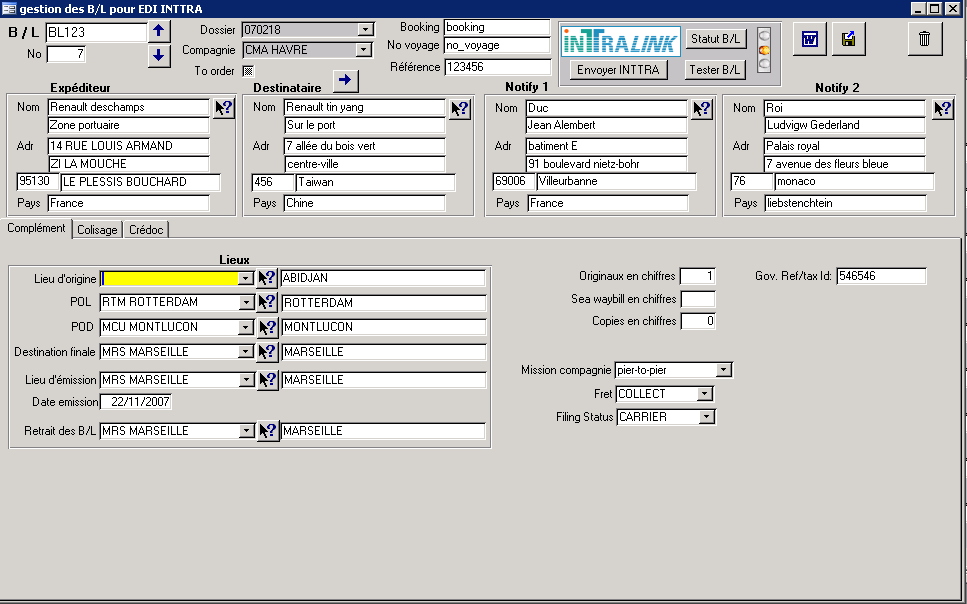
\includegraphics[scale=.9, angle=90]{Contenu/Annexes/Images/FormBL_1.png}
	\end{center}

	\caption{Capture numéro 1}
\end{figure}
\begin{figure}
	\begin{center}
		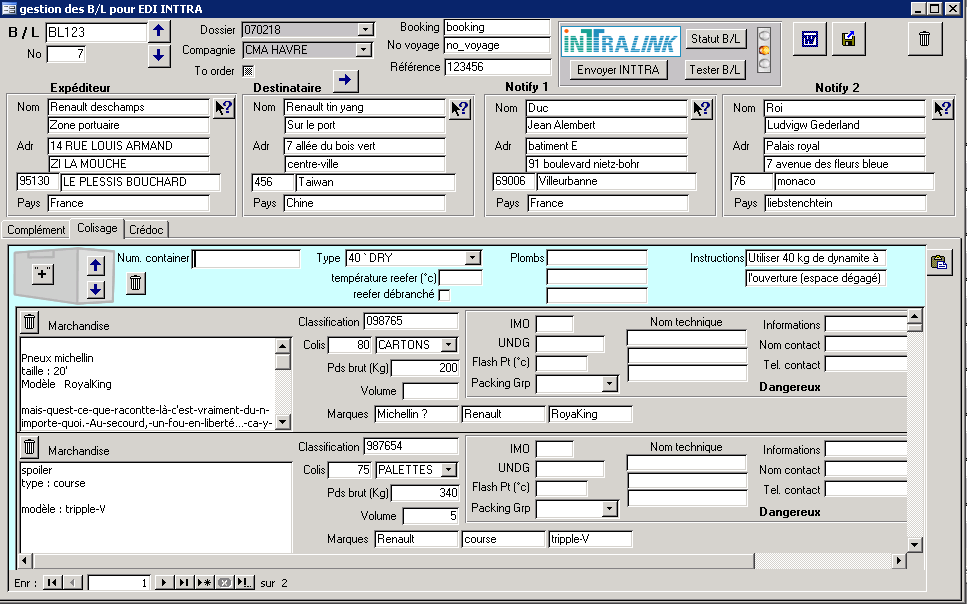
\includegraphics[scale=.9, angle=90]{Contenu/Annexes/Images/FormBL_2.png}
	\end{center}

	\caption{Capture numéro 2}
\end{figure}

\end{document}
